
Hasta este punto se tiene la biblioteca publicada en el gestor de paquetes NPM, pero aún no se tiene conciencia sobre la diferencia que existe entre usar esta biblioteca o implementar React de manera normal.
A continuación se tiene un ejemplo de cómo se implementaría el Front-End para mostrar la lista de calificaciones de un grupo de estudiantes con React.

Queremos tener una vista que tenga el título “Lista de calificaciones” con una tabla que tenga el nombre, el semestre y tres calificaciones parciales. 

Supongamos que al hacer una petición al servidor Back-end ( Esta biblioteca no cubre la manera directa de interactuar con el Back-end ), y nos regresa como respuesta un array con los datos y calificaciones de los alumnos como se muestra en la siguiente imagen,el array llamado ALUMNOS. También tenemos un array llamado HEADER el cual tiene la cabecera de la tabla.

 \newline
     \begin{figure}[H]
    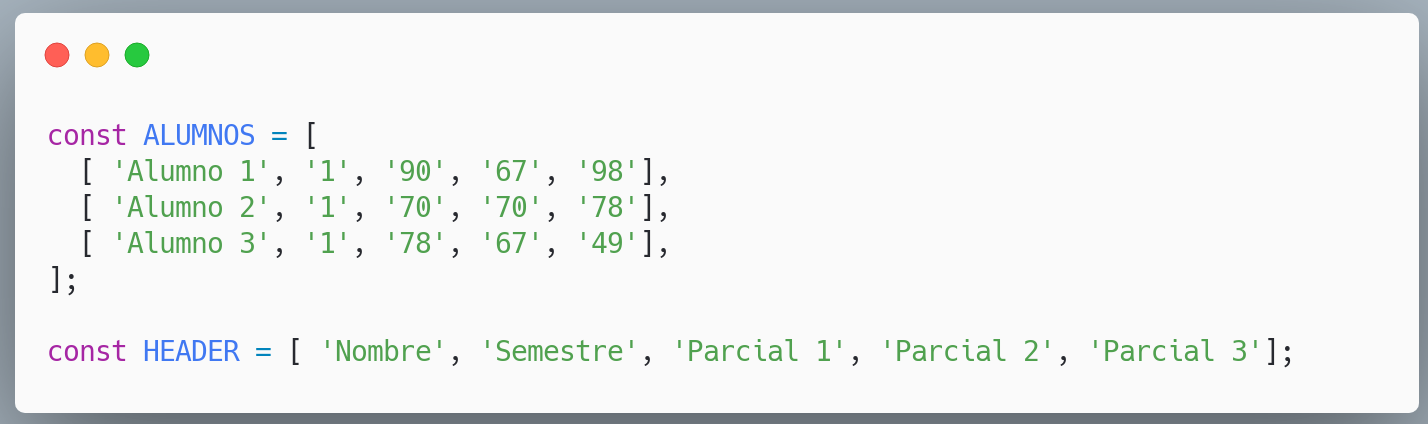
\includegraphics[width=1\textwidth]{./Imagenes/array.png}
     \caption[Crear nuevos directorios]{Array de datos}
         \end{figure}
    \newline

En React tendríamos el siguiente código para poder mostrar en pantalla una tabla.

 \newline
     \begin{figure}[H]
    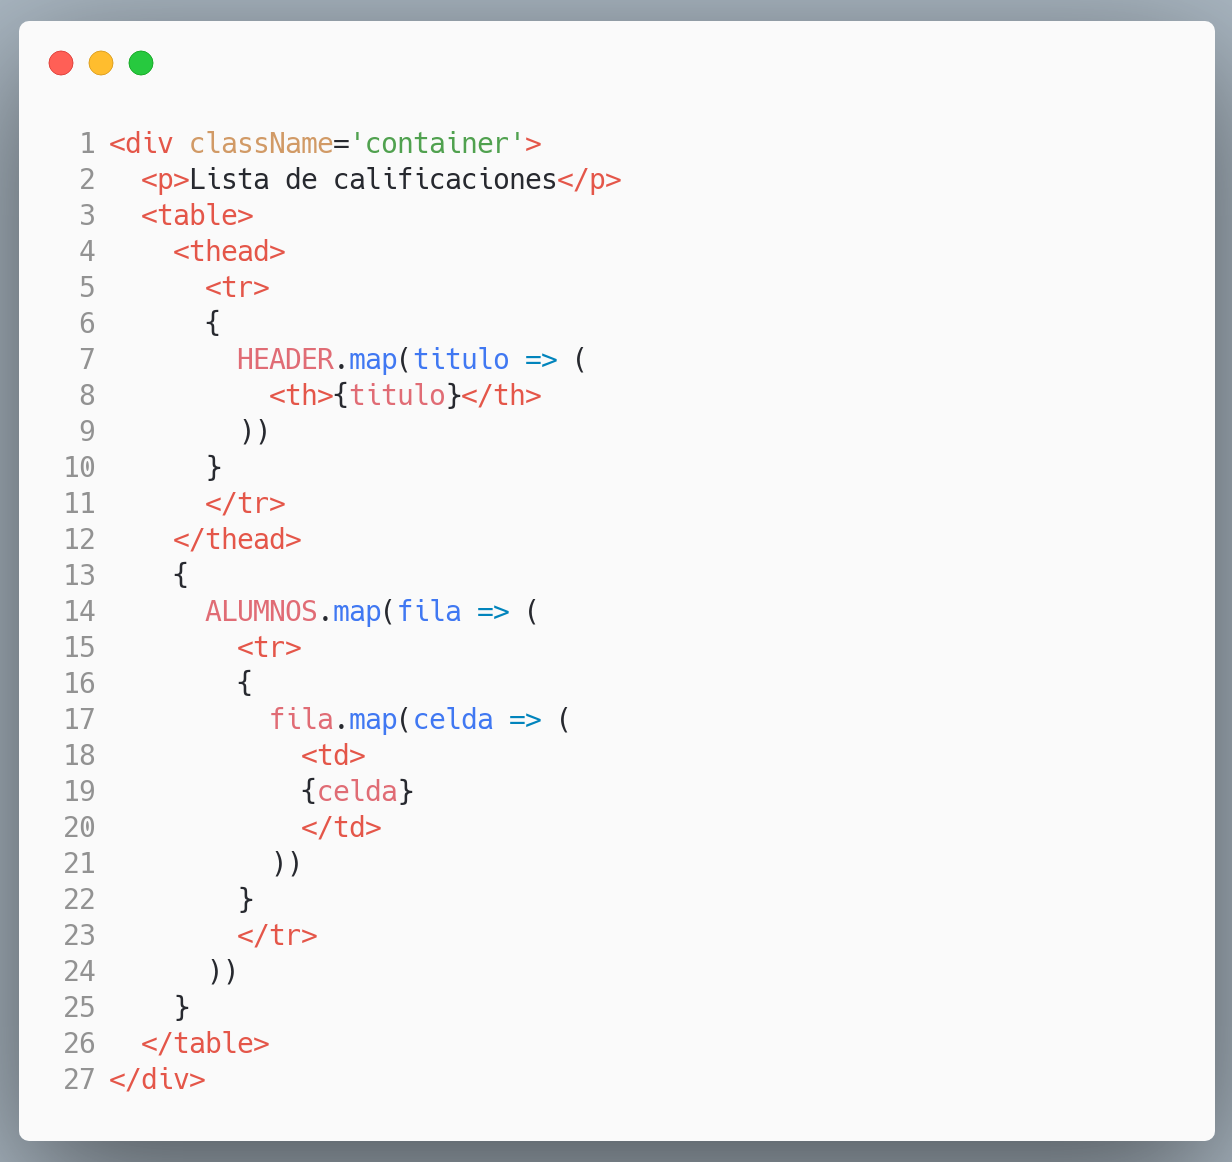
\includegraphics[width=1\textwidth]{./Imagenes/table-react.png}
     \caption[Crear nuevos directorios]{Array de datos}
         \end{figure}
    \newline
    
    En la línea dos, tenemos el título de la vista, a partir de la línea tres tenemos la tabla, la primera parte ( línea cuatro) hacemos la cabecera de la tabla, para esto tenemos que recorrer el array llamado HEADER con ayuda de la función de JavaScript llamada map.

Después en la línea trece, formamos el contenido de la tabla, tenemos que recorrer el array ALUMNOS, primero se recorre fila por fila, y en la línea diecisiete dada una fila, se recorre celda por celda.

Para que esto luzca de manera deseada se tiene el siguiente CSS.

 \newline
     \begin{figure}[H]
    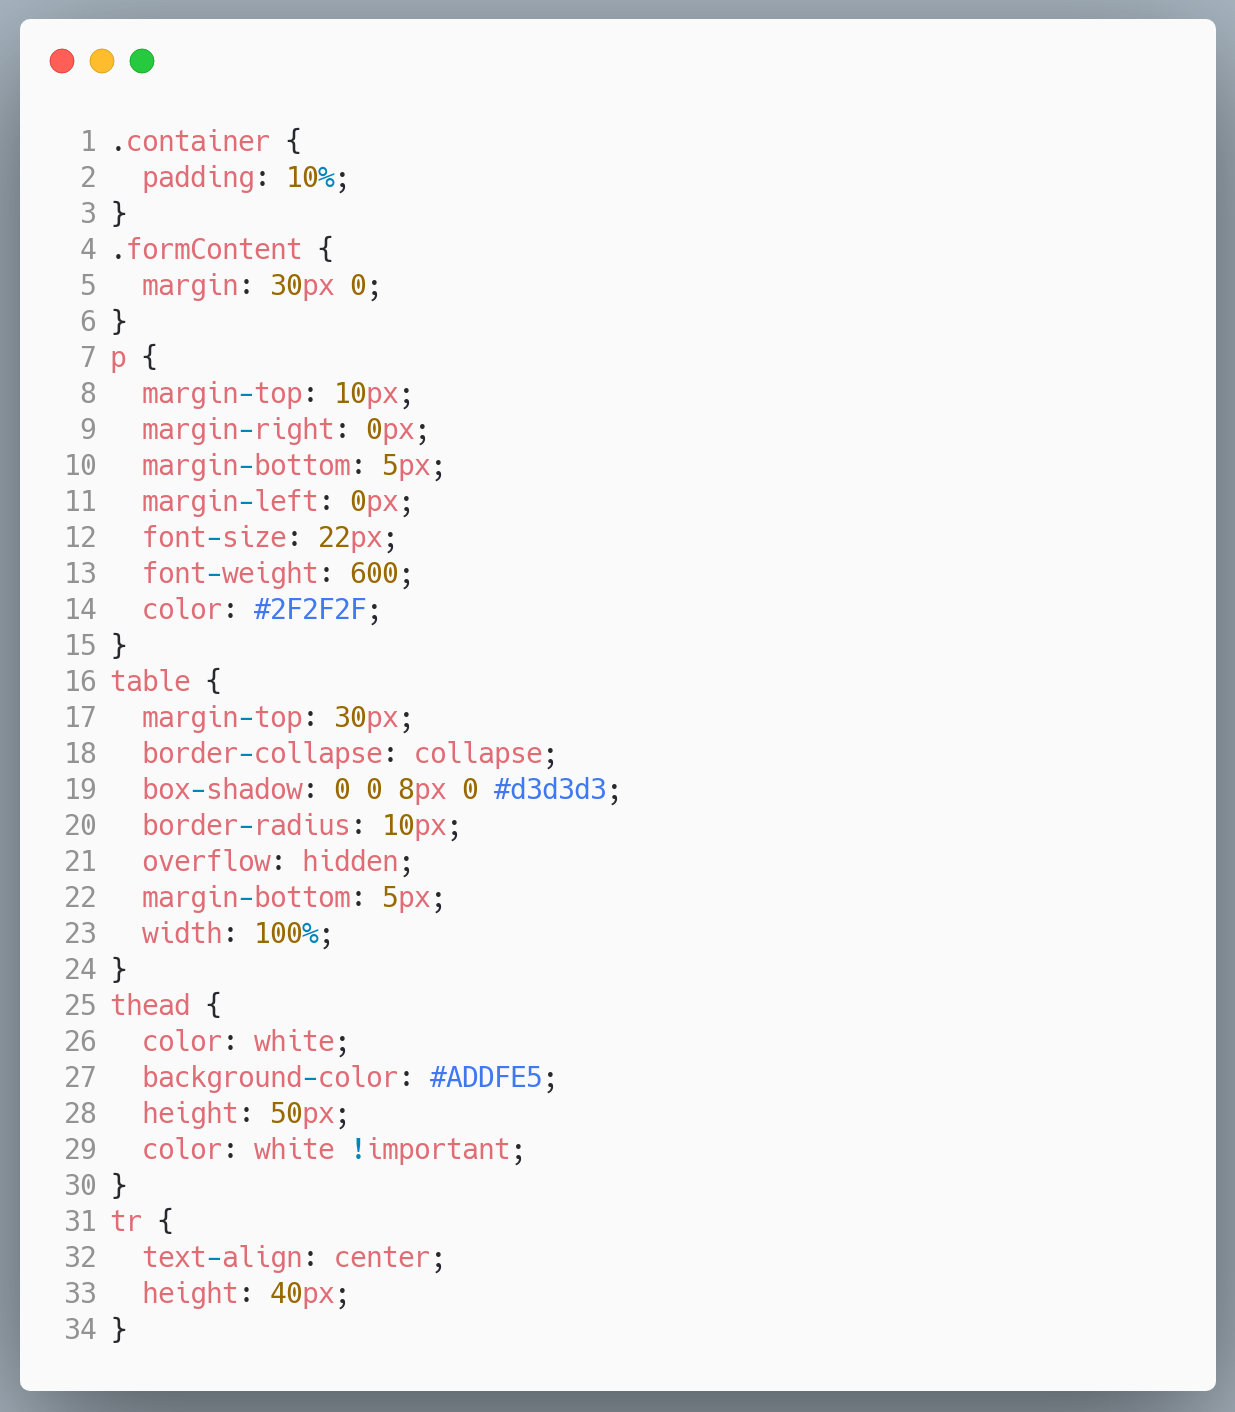
\includegraphics[width=1\textwidth]{./Imagenes/table-css.png}
     \caption[Crear nuevos directorios]{Array de datos}
         \end{figure}
    \newline
    
    Y así tenemos el siguiente resultado.
    
     \newline
     \begin{figure}[H]
    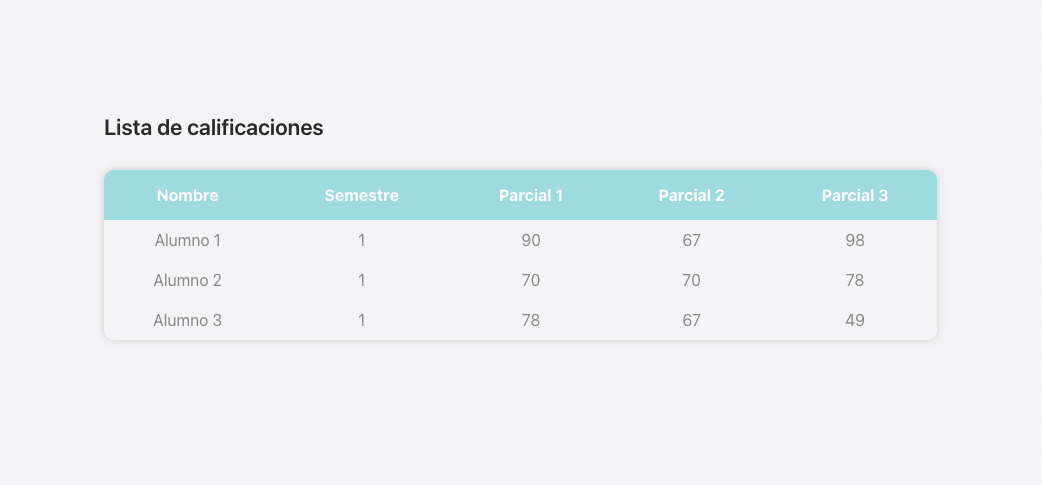
\includegraphics[width=1\textwidth]{./Imagenes/table-res.png}
     \caption[Crear nuevos directorios]{Array de datos}
         \end{figure}
    \newline
    
    Con nuestra biblioteca evitamos el trabajo de formar desde cero la tabla, y no se tiene que dar estilos  CSS, Para tener el resultado anterior no tenemos que hacer nada, más que pasarle los datos de la cabecera y el cuerpo de la tabla de la siguiente manera.
         \newline
     \begin{figure}[H]
    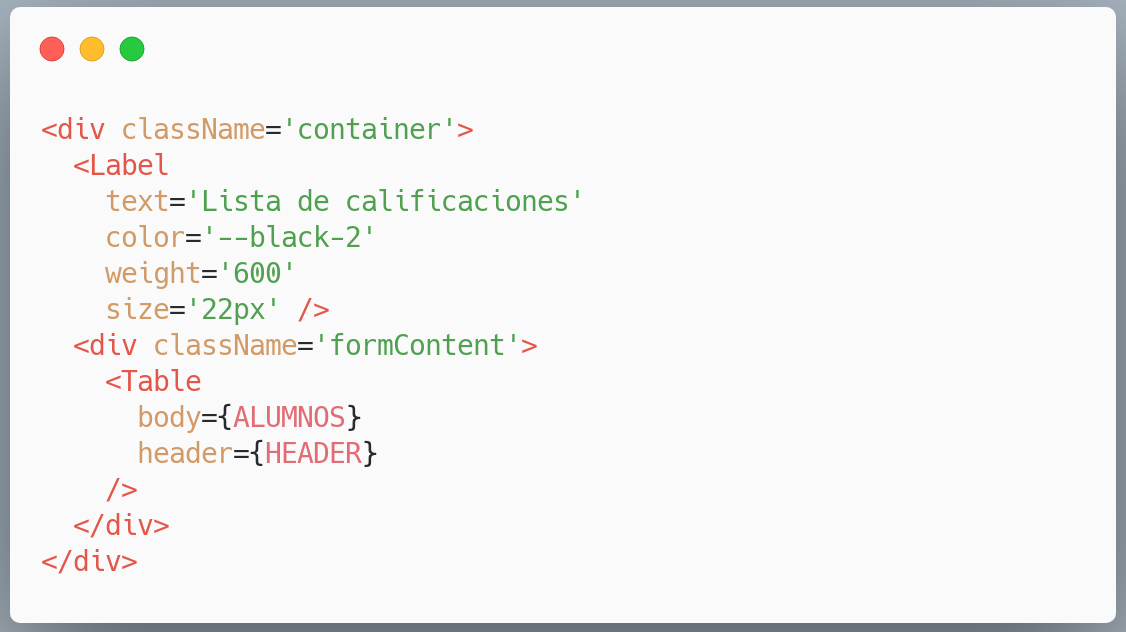
\includegraphics[width=1\textwidth]{./Imagenes/table-crown.png}
     \caption[Crear nuevos directorios]{Array de datos}
         \end{figure}
    \newline
    
    Con el código anterior, estamos usando la biblioteca aquí desarrollada, al inicio tenemos el componente Label al cual le damos parámetros como el tamaño de la letra, su peso y el texto a mostrar que en este caso es “Lista de calificaciones”. Y después tenemos el componente Table, al cual solo le pasamos los arrays ALUMNOS para el cuerpo de la tabla y HEADER para la cabecera de la tabla.
    
    